\documentclass[a4paper, 10pt]{article}
\usepackage[utf8]{inputenc} % Change according your file encoding
\usepackage{graphicx}
\usepackage{url}
\usepackage{amsmath}
\usepackage{mathtools}
\usepackage{amsfonts}
\usepackage{bbm}
\usepackage{amsthm}
\usepackage{fancyhdr}
\usepackage{setspace}
\usepackage{tikz}
\usetikzlibrary{arrows,positioning}
\usepackage[a4paper, left=2cm, right=2cm, top=2.5cm, bottom=2cm]{geometry}

\pagestyle{fancy}
\fancyhf{}
\rhead{Tuesday, December 10th}
\lhead{Mat\'in, Oviedo, and Segarra - DAG: Sheet 1}
\cfoot{\thepage}

\newtheorem{obs}{Observation}
\newtheorem{theorem}{Theorem}
\newtheorem*{theoremstar}{Theorem}

\theoremstyle{definition} % amsthm only
\newtheorem{definition}{Definition}

%\newtheorem{def}{Definition}

\begin{document}
\onehalfspacing
\tikzstyle{vertice}=[circle, draw, fill=black!50, inner sep = 0pt, minimum width=4pt]

\textbf{\Large Discrete and Algorithmic Geometry: Sheet 1}

\vspace{20pt}

\textbf{\textit{(1) Let $M$ be a matroid on the ground set $[n] = \lbrace 1, 2, \dots, n \rbrace$ with family of independent sets $\lbrace I : I \in \mathcal{I}\rbrace$:}}

\vspace{3pt}

\hspace{5pt} \textbf{\textit{(a) Contracion in $M$ as defined in class agrees with the notion of contraction in graphs.}}

\vspace{3pt}

WRITE HERE

\hspace{5pt} \textbf{\textit{(b) Contracion in $M$ as defined in class agrees with $M / S \coloneqq (M^\star \backslash S)^\star$ for a subset $S \subset [n]$.}}

\vspace{3pt}

WRITE HERE

\vspace{3pt}

\hspace{5pt} \textbf{\textit{(c) $M_{G^\star} = \left(M_G\right)^\star$, if G is a planar graph and $G^\star$ its dual planar graph.}}

%\textbf{\textit{(2) Prove that if a matroid M is realizable over a ground field $\mathbbm{k}$, then the dual matroid $M^\star$ is also realizble over $\mathbbm{k}$.}}

\vspace{3pt}

WRITE HERE

\vspace{3pt}

\hspace{5pt} \textbf{\textit{(d) Consider the matroid M realized by the columns of the matrix}}
$$
A = \left[
    \begin{array}{ccccc}
        0 & 1 & 1 & 0 & 1 \\
        1 & 0 & 1 & 0 & 1 \\
        0 & 1 & 1 & 1 & 0
    \end{array}
\right]
$$
\textbf{\textit{Compute a realization of $M^\star$, and some contractions of M of your choosing. Compute the set of circuits and cocircuits of $M$ and of $M^\star$.}}

\vspace{5pt}

We will first compute a realization of matrix A.
To do so, we will swap columns two and four and perform a change of basis to basis $\mathcal{B} = \left\lbrace \left( \begin{array}{c} 0 \\ 1 \\ 0 \end{array} \right), \left( \begin{array}{c} 1 \\ 0 \\ 1 \end{array} \right), \left( \begin{array}{c} 1 \\ 1 \\ 1 \end{array} \right) \right\rbrace$. We then have,
\begin{equation*}
    \begin{split}
        A & = \left[
            \begin{array}{ccccc}
                0 & 1 & 1 & 0 & 1 \\
                1 & 0 & 1 & 0 & 1 \\
                0 & 1 & 1 & 1 & 0
            \end{array}
        \right]
        \longrightarrow
        \left[
            \begin{array}{ccccc}
                0 & 0 & 1 & 1 & 1 \\
                1 & 0 & 1 & 0 & 1 \\
                0 & 1 & 1 & 1 & 0
            \end{array}
        \right]
        \overset{\mathcal{B}}{\longrightarrow}
        \bar{A} = \left[
            \begin{array}{ccccc}
                1 & 0 & 0 & -1 & 0 \\
                0 & 1 & 0 & 0 & -1 \\
                0 & 0 & 1 & 1 & 1
            \end{array}
        \right]
        \hspace{10pt} \text{ which also represents $M$.} \\[10pt]
        \bar{A}B^T & = 0 \Longrightarrow 
        B^T = \left[
            \begin{array}{cc}
                -1 & 0  \\
                0  & -1 \\
                1  & 1 \\
                -1 & 0 \\
                0 & -1
            \end{array}
        \right] \hspace{5pt} \text{ (for example) } \Longrightarrow
        B = \left[
            \begin{array}{ccccc}
                -1 & 0 & 1 & -1 & 0 \\
                0 & -1 & 1 & 0 & -1
            \end{array} 
        \right] \hspace{5pt} \text{ which is $M^*$.}
    \end{split}
\end{equation*}

Now we will compute a contraction of $M$, $M / 1$, using a deletion in its dual matroid, $M^*$, $(M^* \backslash 1)^*$.
\begin{equation*}
    \begin{split}
        B \backslash 1 & = \left[
            \begin{array}{cccc}
                0 & 1 & -1 & 0 \\
                -1 & 1 & 0 & -1 
            \end{array} 
        \right] \text{ ;} \hspace{5pt}
        (B  \backslash 1)\cdot c^T = 0 \Rightarrow 
        c^T = \left[
                \begin{array}{cc}
                    0 & 1 \\
                    1 & 1 \\
                    1 & 1 \\
                    1 & 0
                \end{array} 
            \right] \Rightarrow
        c = \left[
                \begin{array}{cccc}
                    0 & 1 & 1 & 1 \\
                    1 & 1 & 1 & 0
                \end{array} 
            \right] \hspace{3pt} \text{which is $M / 1$.}
    \end{split}
\end{equation*}

An alternative method for computing $ M / 1$ is doing the projection in the corresponding direction. In particular, to find $ M / 1$ it suffices to project $A$ in direction $\left( \begin{array}{ccc} 0 & 1 & 0 \end{array} \right)^T$ and get rid of loops. In particular,
\begin{equation*}
    \begin{split}
        A & = \left[
            \begin{array}{ccccc}
                0 & 0 & 1 & 1 & 1 \\
                1 & 0 & 1 & 0 & 1 \\
                0 & 1 & 1 & 1 & 0
            \end{array}
        \right]
        \overset{\text{\footnotesize{Project}}}{\longrightarrow}
        \left[
            \begin{array}{ccccc}
                0 & 0 & 1 & 1 & 1 \\
                0 & 1 & 1 & 1 & 0
            \end{array}
        \right]
        \overset{\text{\footnotesize{No Loops}}}{\longrightarrow}
        \left[
            \begin{array}{ccccc}
                0 & 1 & 1 & 1 \\
                1 & 1 & 1 & 0
            \end{array}
        \right] \hspace{5pt} \text{ which again is $ M / 1$.}
    \end{split}
\end{equation*}

Lastly, circuits are minimal linear combinations, and co-circuits are their dual counterparts.
Hence, computing both the circuits of $M$ and $M^*$ we will also have the co-circuits of $M^*$ and $M$ respectively.
In particular, by inspection we have:
\begin{equation*}
    \text{Circuits of $M$ } = (-1, 0, 1, -1, 0), (0, -1, 1, 0, -1) = \text{ Cocircuits of $M^*$}
\end{equation*}
\begin{equation*}
    \text{Circuits of $M^*$ } = (1, 1, 1, 0, 0), (0, 0, 1, 1, 1), (1, 0, 0, -1, 0), (0, 1, 0, 0, -1) = \text{ Cocircuits of $M$}
\end{equation*}


\vspace{5pt}

\begin{center}
    \rule{5cm}{0.4pt}
\end{center}

\newpage

\textbf{\textit{(2) Let $A \in \mathbb{R}^{n\times d}$ be a matrix of full rank, and let the columns of $B \in \mathbb{R}^{n \times (n -d)}$ be a basis of the row space of $A$, so that $AB = 0$ and the rows of $B$ are a Gale transform of the columns of $A$. We saw in class that $\text{LinVal}(A) = \text{LinDep}(B)$. Show that $\text{LinVal}(B) = \text{LinDep}(A)$.}}

\vspace{3pt}

WRITE HERE


\vspace{5pt}

\begin{center}
    \rule{5cm}{0.4pt}
\end{center}

\newpage

\textbf{\textit{(3) The greedy algorithm always works for matroids.}}

\hspace{5pt}\textbf{\textit{(a) Show that Kruskal's greedy algorithm always finds a maximum weight independent set in a matroid $M = (E, \mathcal{I})$, regardless of the choice of weight function $\omega : E \mapsto \mathbb{R}_{>0}$. Recall that the greedy algorithm starts by setting $I \coloneqq \emptyset$, and next repeatedly chooses $y \in E \backslash I$ with $I \cup \lbrace y \rbrace \in \mathcal{I}$ and with $\omega(y)$ as large as possible. It stops if no such $y$ exists.}}

\vspace{3pt}

Let us rename the independent sets $I_0, I_1, \ldots, I_r$, where $I_0 = \emptyset$, and $I_{j+1} = I_j \cup \{y_j\}$, for some $y_j \in E \setminus I_j$ with $\omega y_j$ as large as possible. Let us show $|I_j| = j$ by induction, and that, assuming $E$ is finite, there exists a final $I_r$, for some $r$ that satisfies $r = \max_{I \in \mathcal I} |I|$.

For $j = 0$, $|I_0| = |\emptyset| = 0$
For $j > 0$, assuming induction hypothesis, $I_{j+1} = I_j \cup \{y_j\}$, for some $y_j \in E \setminus I_j$, and therefore $|I_{j+1}| = |I_j| + 1 = j + 1$. Assume that the last independendent set is $I_s$ for some $s$. Obviously, $s \leq r = \max_{I \in \mathcal I} |I|$, since $I_s \in \mathcal I$. If $s < r$, there will be a set $I'$ with $|I'| = r$. By the exchange axiom, there would be an $y_s \in I' \setminus I_s \subset E \setminus I_s$ such that $I_s \cup \{y_s\} \in \mathcal I$, leading to a contradiction since $|I_s \cup \{y_s\} \in \mathcal I| = s + 1 > s$.

We are left with proving that the weight we obtain with the algorithm is indeed the maximum achievable. Let us show by induction that $I_j$ is contained in an optimal basis $B$.

For the case $j = 0$, it is trivial, since $\emptyset = I_0 \subset B$. Now, applying induction hypothesis, if $I_j \subset B$, let us see what happens for $I_{j+1} = I_j \cup \{y_j\}$. If $y_j \in B$, $I_{j+1} \subset B$, so let us assume $y_j \notin B$. In this case $I_{j+1} \not\subset B$, but $I_{j+1} \subset B'$ for some basis $B'$ which is not optimal. By the exchange axiom, since $y_j \in B' \setminus B$, there is $y_j' \in B \setminus B'$ such that $B'' = B \setminus \{y_j'\} \cup \{y_j\}$ is a basis. $I_j \cup \{y_j'\}$ is independent as well since it is contained in a basis. By the construction of the algorithm, $\omega(y_j') \leq \omega(y_j)$. This implies that
\[
\sum_{b \in B} \omega(b) =
w(y_j') + \sum_{b \in B, b \neq y_j'} \omega(b) \leq
w(y_j) + \sum_{b \in B, b \neq y_j} \omega(b) =
\sum_{b \in B \setminus \{y_j'\} \cup \{y_j'\}} \omega(b) =
\sum_{b \in B''} \omega(b),
\]
Meaning that $B''$ is another optimal basis that contains $I_{j+1}$.

Finally, $I_r$, since its size will be the maximum set of an independent set, and therefore is a basis. Since a basis cannot be contained in another basis, $I_r$ will be the optimal basis.
\vspace{3pt}

\hspace{5pt}\textbf{\textit{(b) Show that that this property characterizes independent sets of matroids among all simplicial complexes. In other words, given a simplicial complex $\Sigma$ for which the greedy algorithm always works, regardless of the weight function~$\omega$, show that $\Sigma = \mathcal I(M)$ for some matroid~$M$.}}

\vspace{3pt}

WRITE HERE


\vspace{5pt}

\begin{center}
    \rule{5cm}{0.4pt}
\end{center}

\newpage

\textbf{\textit{(4) Using a famous result by Jack Edmonds, prove the following:}}

\hspace{5pt}\textbf{\textit{(a) Let $G=(V,E)$ be a bipartite graph with color classes $V_1,V_2$. For $i=1,2$, let $M_i$~be the matroid where $I\subseteq E$ is independent if and only if each vertex in~$V_i$ is covered by at most one edge in~$I$. Use the Matroid Intersection Theorem to prove:}}
    \begin{theoremstar}[K\H onig's Matching Theorem]
      The maximum size of a matching in a bipartite graph equals the minimum size of a vertex cover.
    \end{theoremstar}

\vspace{3pt}

WRITE HERE

\vspace{3pt}

\hspace{5pt}\textbf{\textit{(b) Let $G=(V,E)$ be a graph whose edges are partitioned into $k$~colors, $E=E_1\cup E_2\cup\cdots\cup E_k$. Use the Matroid Intersection Theorem to prove that there exists a rainbow spanning tree (a spanning tree all of whose edges are colored differently) if and only if $G-F$ has at most $t+1$ connected components, for any union~$F$ of $t$~colors, for any $t\ge0$.}}

\vspace{3pt}

WRITE HERE


\vspace{5pt}

\begin{center}
    \rule{5cm}{0.4pt}
\end{center}

\newpage

\textbf{\textit{(5) Let $\cT=\{\sigma_1,\dots,\sigma_m\}$ be a triangulation of a full-dimensional point configuration $\cA=(\aaa_1,\dots,\aaa_n)\subset\RR^d$ of $n$~points, where we consider the $\sigma_i\in\binom{[n]}{d+1}$ to be index sets. Let $R^{\text{int}}$ be the set of interior ridges, defined to be intersections $\rho = \rho_{ij} = \sigma_i\cap\sigma_j$ of two facets of~$\cT$ such that the affine span of the points of~$\cA$ indexed by~$\rho$ has dimension~$d-1$. (In the triangulations of~Figure~\ref{fig:triangs1}, they are the interior edges.)}}

  \begin{figure}[htbp]
    \centering
    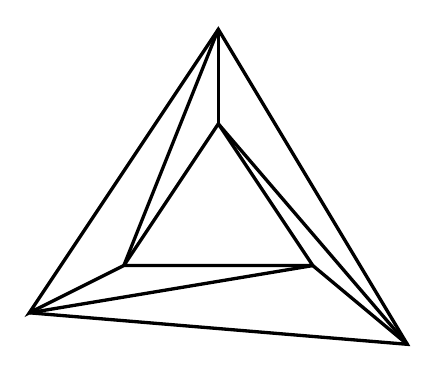
\begin{tikzpicture}[scale=.4]
      \coordinate (1) at (0,0);
      \coordinate (2) at (12,-1);
      \coordinate (3) at (6,9);
      \coordinate (4) at (3,1.5);
      \coordinate (5) at (9,1.5);
      \coordinate (6) at (6,6);

      \draw[very thick] (1)--(2)--(3)--(1)--(4)--(5)--(6)--(4);
      \draw[very thick] (2)--(5);
      \draw[very thick] (3)--(6);

      \draw[very thick] (1)--(5);
      \draw[very thick] (2)--(6);
      \draw[very thick] (3)--(4);
    \end{tikzpicture}
    \qquad
    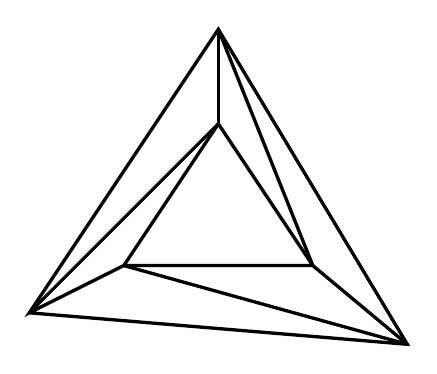
\begin{tikzpicture}[scale=.4]
      \coordinate (1) at (0,0);
      \coordinate (2) at (12,-1);
      \coordinate (3) at (6,9);
      \coordinate (4) at (3,1.5);
      \coordinate (5) at (9,1.5);
      \coordinate (6) at (6,6);

      \draw[very thick] (1)--(2)--(3)--(1)--(4)--(5)--(6)--(4);
      \draw[very thick] (2)--(5);
      \draw[very thick] (3)--(6);

      \draw[very thick] (2)--(4);
      \draw[very thick] (3)--(5);
      \draw[very thick] (1)--(6);
    \end{tikzpicture}    
    \caption{Two triangulations.
    View the source code for the coordinates of the points.}
    \label{fig:triangs1}
  \end{figure}

\begin{enumerate}
  \item
    For a vector $\omega\in\RR^n$, lift the points in $\cA$ to heights~$\omega$, so that
    $\cA^\omega=\big(\binom{\aaa_1}{\omega_1},\dots,\binom{\aaa_n}{\omega_n}\big)$.
    For each interior ridge $\rho=\sigma_i\cap\sigma_j\in R^{\text{int}}$,
    formulate the folding condition that expresses that $\rho$ indexes a face of the lower convex hull of~$\cA^\omega$,
    in terms of the coordinates of the~$\aaa_i$ and~$\omega$.
    Your folding condition should be an inequality that is linear in each height~$\omega_i$.

To formulate the folding condition, we make use of Definition 7.4 in Rheka R. Thomas~\footnote{Rekha R. Thomas. Lectures in geometric combinatorics., volume 33 of Student Mathematical Library. Providence, RI: American Mathematical Society (AMS); Princeton, NJ: Institute for Advanced Studies, 2006.}:
        \begin{equation*}
            bla
        \end{equation*}

  \item
    Write code that takes the coordinates of the $\aaa_i$ and the facets $\sigma_i$ of a triangulation as input,
    and outputs the set of folding conditions in a text file in
    LP file format.

  \item
    Download a linear programming software such as
    \texttt{gurobi},
    \texttt{cplex} or
    \texttt{scip}/\texttt{soplex}
    and check explicitly whether there exists a choice of heights $\omega$ that induces each of the triangulations of Figure~\ref{fig:triangs1}.

  \item
    Using this code,
    check that the triangulation of the $4$-dimensional cube from~\cite{deLoera96}
    given by the files \texttt{4-cube.vertices} and \texttt{4-cube.triangulation}
    is non-regular, i.e., it does not come from a lifting to~$\RR^5$.
    If you like, download and play with TOPCOM.
  \end{enumerate}


\vspace{5pt}

\begin{center}
    \rule{5cm}{0.4pt}
\end{center}

\vspace{5pt}

\end{document}
